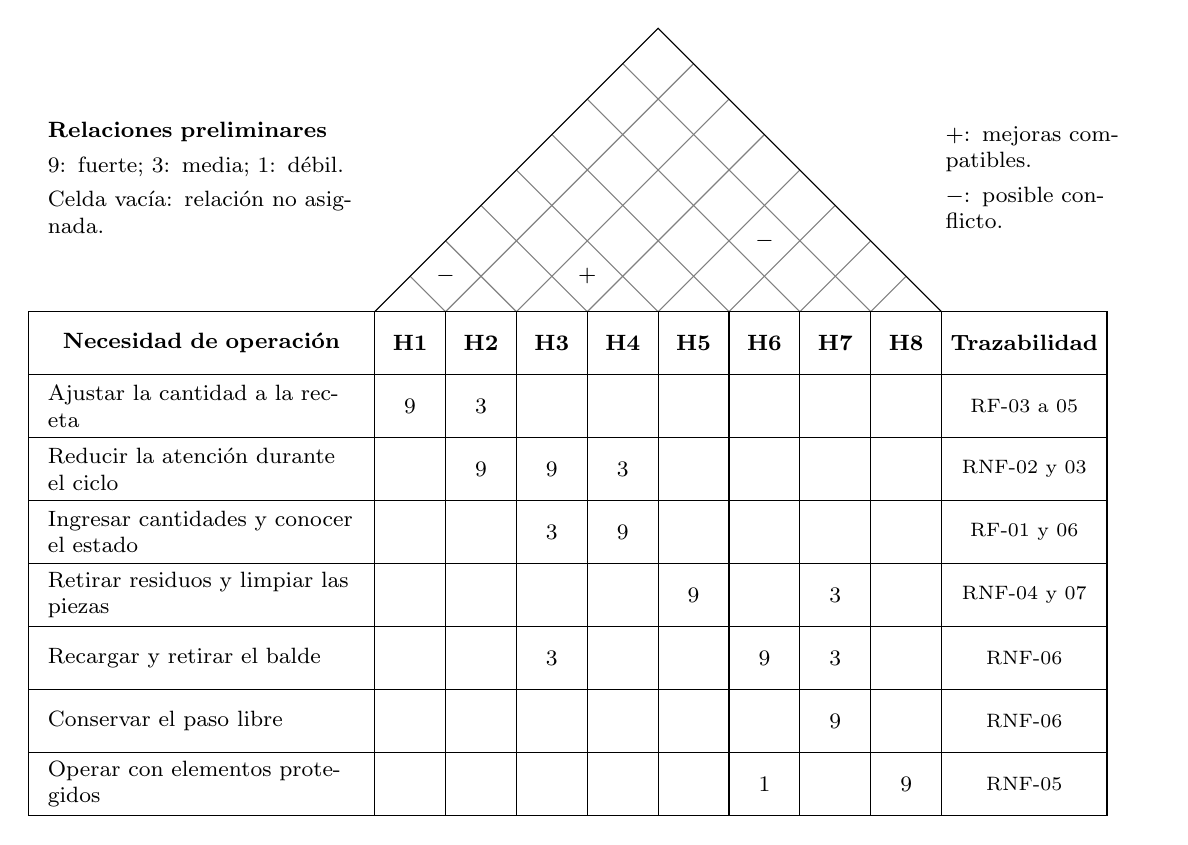
\begin{tikzpicture}[font=\footnotesize]
    % H1--H8: características definidas en la tabla de lectura de la casa.
    \begin{scope}
        \clip (0,0) -- (7.2,0) -- (3.6,3.6) -- cycle;
        \foreach \k in {0,...,8} {
            \draw[gray] (\k*0.9,0) -- ++(3.6,3.6);
            \draw[gray] (\k*0.9,0) -- ++(-3.6,3.6);
        }
    \end{scope}
    \draw (0,0) -- (3.6,3.6) -- (7.2,0);
    % Conflictos/compatibilidades propuestos, sujetos a revisión técnica.
    \node at (0.9,0.45) {$-$};       % H1 frente a H2
    \node at (2.7,0.45) {$+$};       % H3 frente a H4
    \node at (4.95,0.90) {$-$};      % H5 frente a H7
    \draw (-4.4,0) rectangle (9.3,-6.4);
    \draw (0,0) -- (0,-6.4);
    \draw (7.2,0) -- (7.2,-6.4);
    \foreach \k in {1,...,7} {\draw (\k*0.9,0) -- (\k*0.9,-6.4);}
    \foreach \k in {1,...,8} {\draw (-4.4,-\k*0.8) -- (9.3,-\k*0.8);}
    \node[align=center,text width=40mm] at (-2.2,-0.4) {\textbf{Necesidad de operación}};
    \node[align=center] at (8.25,-0.4) {\textbf{Trazabilidad}};
    \foreach \k in {1,...,8} {\node at ({(\k-0.5)*0.9},-0.4) {\textbf{H\k}};}
    \foreach \y/\texto/\rf in {
        1.2/{Ajustar la cantidad a la receta}/{RF-03 a 05},
        2.0/{Reducir la atención durante el ciclo}/{RNF-02 y 03},
        2.8/{Ingresar cantidades y conocer el estado}/{RF-01 y 06},
        3.6/{Retirar residuos y limpiar las piezas}/{RNF-04 y 07},
        4.4/{Recargar y retirar el balde}/{RNF-06},
        5.2/{Conservar el paso libre}/{RNF-06},
        6.0/{Operar con elementos protegidos}/{RNF-05}}
    {
        \node[align=left,text width=39mm] at (-2.2,-\y) {\texto};
        \node[align=center,text width=19mm,font=\scriptsize] at (8.25,-\y) {\rf};
    }
    % Relaciones 9/3/1: juicio preliminar de diseño, no resultados medidos.
    \foreach \r/\c/\v in {
        1/1/9,1/2/3,
        2/2/9,2/3/9,2/4/3,
        3/3/3,3/4/9,
        4/5/9,4/7/3,
        5/3/3,5/6/9,5/7/3,
        6/7/9,
        7/6/1,7/8/9}
    {\node at ({(\c-0.5)*0.9},{-(\r+0.5)*0.8}) {\v};}
    \node[align=left,text width=39mm] at (-2.2,1.7)
        {\textbf{Relaciones preliminares}\\[3pt]9: fuerte; 3: media; 1: débil.\\[3pt]Celda vacía: relación no asignada.};
    \node[align=left,text width=26mm] at (8.55,1.7)
        {$+$: mejoras compatibles.\\[3pt]$-$: posible conflicto.};
\end{tikzpicture}
